\title{EL TIEMPO PASA, Y EL SOFTWARE MUERE}

\author{Ignacio Slater}
\newcommand{\subtitle}{Cómo diseñar programas resistentes al cambio}
\affil{Departamento de Ciencias de la Computación, Universidad de Chile}

\date{\today}


\newtheorem{theorem}{Theorem}
\newtheorem*{note}{Nota}
\newtheorem*{important}{Importante}
\theoremstyle{definition}
\newtheorem{definition}{Definición}[chapter]
\newtheorem{exercise}[definition]{Ejercicio}
\definecolor{LightGray}{gray}{0.9}
\definecolor{Transparent}{gray}{1.0}
 
\setlength\epigraphwidth{\textwidth}

%%
 % Java inline source code
 %%
\newcommand{\java}[1]{\mintinline{java}{#1}}

% | Creates an index from text and renders the text.
\newcommand{\idx}[1]{#1\index{#1}}

% | Creates an index from text and renders the text in italics.
\newcommand{\idxit}[1]{\textit{#1}\index{#1}}

% | Inserts a figure in the document
% | 
% | Arguments:
% |   #1: the position of the figure (float)
% |   #2: the path to the image
% |   #3: the caption of the figure
% |   #4: the label of the figure
% |   #5: \includegraphics options
\newcommand{\insertFigure}[3][]{
   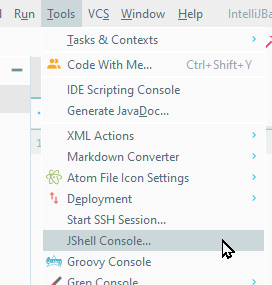
\includegraphics[width=0.6\textwidth]{Por_algo_se_empieza/idea64_tools_jshell.png}
   \caption{Acceso a la consola \textit{JShell}}
}

% | Horizontal rule with text in the middle.
\newcommand*\ruleline[1]{\par\noindent\raisebox{.8ex}{\makebox[\linewidth]{\hrulefill\hspace{1ex}\raisebox{-.8ex}{#1}\hspace{1ex}\hrulefill}}}

% | tcolorbox environment with enhanced borders, breakable content, and a title.
\newtcolorbox{defaultbox}[1][]{enhanced, breakable, title=#1}

\newtcolorbox[auto counter,number within=chapter]{ejercicio}[2][]{
  enhanced, 
  breakable, 
  title=¡Te toca!\hfill (#2 \thetcbcounter), 
  colback=Black!5!white, 
  colframe=Black!75!black,
  #1
}

\newtcblisting{powershell}{
   enhanced,
   breakable,
   listing engine=minted,
   minted style=emacs,
   minted language=powershell,
   minted options={autogobble},
   colback=blue!5!white,
   colframe=Cerulean!75!black,
   listing only,
   left=5mm,enhanced,
   overlay={
      \begin{tcbclipinterior}
         \fill[Cerulean!20!white] (frame.south west) rectangle ([xshift=5mm]frame.north west);
      \end{tcbclipinterior}
   }
}

\newtcblisting{bash}{
   enhanced,
   breakable,
   listing engine=minted,
   minted style=perldoc,
   minted language=bash,
   minted options={autogobble},
   colback=blue!5!white,
   colframe=Emerald!75!black,
   listing only,
   left=5mm,enhanced,
   overlay={
      \begin{tcbclipinterior}
         \fill[Emerald!20!white] (frame.south west) rectangle ([xshift=5mm]frame.north west);
      \end{tcbclipinterior}
   }
}

\newtcblisting{kotlin}{
   enhanced,
   breakable,
   listing engine=minted,
   minted style=manni,
   minted language=kotlin,
   minted options={autogobble},
   colback=Orange!5!white,
   colframe=Peach!75!black,
   listing only,
   left=5mm,enhanced,
   overlay={
      \begin{tcbclipinterior}
         \fill[Peach!20!white] (frame.south west) rectangle ([xshift=5mm]frame.north west);
      \end{tcbclipinterior}
   }
}

\newtcblisting{md}{
   enhanced,
   breakable,
   listing engine=minted,
   minted style=trac,
   minted language=markdown,
   minted options={autogobble},
   colback=Gray!5!white,
   colframe=Gray!75!black,
   listing only,
   left=5mm,enhanced,
   overlay={
      \begin{tcbclipinterior}
         \fill[Gray!20!white] (frame.south west) rectangle ([xshift=5mm]frame.north west);
      \end{tcbclipinterior}
   }
}

\newtcblisting{xml}{
   enhanced,
   breakable,
   listing engine=minted,
   minted style=friendly,
   minted language=xml,
   minted options={autogobble},
   colback=Blue!5!white,
   colframe=Blue!75!black,
   listing only,
   left=5mm,enhanced,
   overlay={
      \begin{tcbclipinterior}
         \fill[Blue!20!white] (frame.south west) rectangle ([xshift=5mm]frame.north west);
      \end{tcbclipinterior}
   }
}

\newtcblisting{json}{
   enhanced,
   breakable,
   listing engine=minted,
   minted style=perldoc,
   minted language=json,
   minted options={autogobble},
   colback=Magenta!5!white,
   colframe=Magenta!75!black,
   listing only,
   left=5mm,enhanced,
   overlay={
      \begin{tcbclipinterior}
         \fill[Magenta!20!white] (frame.south west) rectangle ([xshift=5mm]frame.north west);
      \end{tcbclipinterior}
   }
}

\newtcblisting{yaml}{
   enhanced,
   breakable,
   listing engine=minted,
   minted style=trac,
   minted language=yaml,
   minted options={autogobble},
   colback=Green!5!white,
   colframe=Green!75!black,
   listing only,
   left=5mm,enhanced,
   overlay={
      \begin{tcbclipinterior}
         \fill[Green!20!white] (frame.south west) rectangle ([xshift=5mm]frame.north west);
      \end{tcbclipinterior}
   }
}

\let\oldquote\quote
\let\endoldquote\endquote
\renewenvironment{quote}[2][]
  {\if\relax\detokenize{#1}\relax
     \def\quoteauthor{#2}%
   \else
     \def\quoteauthor{#2~---~#1}%
   \fi
   \oldquote}
  {\par\nobreak\smallskip\hfill(\quoteauthor)%
   \endoldquote\addvspace{\bigskipamount}}
   